%%%%%%%%%%%%%%%%%%%%%%%%%%%%%%%%%%%%%%%%%%%%%%%%%%%%%%%
% A template for Wiley article submissions.
% Developed by Overleaf. 
%
% Please note that whilst this template provides a 
% preview of the typeset manuscript for submission, it 
% will not necessarily be the final publication layout.
%
% Usage notes:
% The "blind" option will make anonymous all author, affiliation, correspondence and funding information.
% Use "num-refs" option for numerical citation and references style.
% Use "alpha-refs" option for author-year citation and references style.
\PassOptionsToPackage{author-year,initials,nobysame}{amsrefs}
\documentclass[ams-refs]{wiley-article}
% \documentclass[blind,ams-refs]{wiley-article}

% Add additional packages here if required
\usepackage{siunitx}

% added LG
\usepackage{lineno}
\usepackage{todonotes}
\usepackage{verbatim}

% Update article type if known
\papertype{Original Article}
% Include section in journal if known, otherwise delete
\paperfield{Journal Section}

\title{Not reaching your target: single-trial analysis elucidating spatio-temporal multisensory integration in parietal EEG sources}
% alternative titles
% sources capture sensory prediction errors but are not modulated by ongoing motor behavior
% Single-trial regression mapping biomechanics to event-related brain dynamics: hand movement velocity impacts posterior cingulate activity in sensory-motor coupling
% Not reaching your target: prediction errors are modulated by hand movement speed, haptic feedback 
%mobi using motion parameters to inform brain dynamic analysis
%Sensory-motor integration in anterior cingulate cortex: visuo-haptic mismatches and the impact of hand movement speed

% List abbreviations here, if any. Please note that it is preferred that abbreviations be defined at the first instance they appear in the text, rather than creating an abbreviations list.
%\abbrevs{ABC, a black cat; DEF, doesn't ever fret; GHI, goes home immediately.}

% Include full author names and degrees, when required by the journal.
% Use the \authfn to add symbols for additional footnotes and present addresses, if any. Usually start with 1 for notes about author contributions; then continuing with 2 etc if any author has a different present address.
\author[1\authfn{1}]{Lukas Gehrke}
\author[1]{Sezen Akman}
\author[1]{Marius Klug}
\author[2]{Pedro Lopes PhD}
\author[1,3,4,5]{Klaus Gramann PhD}

%\contrib[\authfn{1}]{Equally contributing authors.}

% Include full affiliation details for all authors
\affil[1]{Biopsychology and Neuroergonomics, Institute of Psychology and Ergonomics, TU Berlin, Berlin, Berlin, 10623, Germany}
\affil[2]{Department, Institution, City, State or Province, Postal Code, Country}

\corraddress{Lukas Gehrke, Biopsychology and Neuroergonomics, TU Berlin, Berlin, Berlin, 10623, Germany}
\corremail{lukas.gehrke@tu-berlin.de}

\presentadd[\authfn{1}]{Biopsychology and Neuroergonomics, Institute of Psychology and Ergonomics, TU Berlin, Berlin, Berlin, 10623, Germany}

\fundinginfo{This research was supported by a grant from the German Federal Ministry of Education and Research (01GQ1511) to KG}

% Include the name of the author that should appear in the running header
\runningauthor{Gehrke et al.}

\begin{document}
\maketitle

% added LG
%\linenumbers

% add abstract
\begin{abstract}

Neural interface technology holds significant promise to track user experience implicitly. Today, it finds increasing application in VR/AR as it allows user assessment without breaking the immersive experience. In VR, designing immersion is the key challenge. Unfortunately, the established metric to assess the effectiveness of immersive VR simulations relies on questionnaires. In this work, we present a complimentary metric based on a Brain-Computer Interface. For the metric to be useful beyond prototypical applications, the neural signal employed must be reliable. Hence, it is beneficial to target the signal's cortical origin directly, separating signal from noise. We designed a reach-to-touch paradigm in VR to probe EEG and movement adaptation to visuo-haptic glitches. Our working hypothesis was, that these glitches, or violations of the predicted action outcome, may indicate a disrupted user experience. The classification scheme using trial-to-trial movement adaptation to classify VR glitches did not exceed chance level performance. However, using Prediction Error EEG features, we classified VR glitches with ~77\% accuracy. We localized the EEG sources driving the classification and found midline cingulate and a distributed network of parieto-occipital EEG sources to enable the classification success. Hence, Prediction Error EEG features from these sources reflect violations of user's predictions during interaction with AR/VR, serving as as a robust, targeted, marker for adaptive user interfaces.

% Please include a maximum of seven keywords
\keywords{EEG, Virtual Reality, BCI, Neural Interface Technology, Post-error Slowing, Prediction Error, Predictive Coding}
\end{abstract}

% add main content
% introduction
\section{Introduction}
In order for brains to accurately infer about the latent variables governing the environment, e.g. gravity, recent theories proclaim that brains set out to actively sample their environment to confirm predictions of prior hypotheses. \cites{Clark2013, Friston2010, Rao1999}. This active sampling is inherently tied to the bodies capabilities to act on the world, rendering the action-perception cycle of cognition a deeply embodied process \cite{Friston2012}. The minimisation of surprise or prediction error, as the incentive of active inference has been extensively studied in relation to perception in motor control. Here, active inference typically considers engaged viewing, saccadic eye movements, as an observable manifestation of how the brain directs motor output during active sampling, i.e. hypothesis testing, of the environment. However, environmental affordances surpass the visual domain. Particularly in humans and apes, a proclivity to use both hands to act on the world emerged and are greatly trusted upon. So much so, that many tasks can be completed without concurrently consulting the visual domain, e.g. typewriting or even reaching for a cup. On the computational level, a "bidirectional cascade of cortical processing" arguably underlies such inferential processing \cite{Clark2013}. A hierarchical generative model, or forward model, of the environment is assumed that is trained to minimize prediction errors from elicited actions, or in other words "actively constructing explanations" \cite{Wolpert2011, Friston2018}.

Simultaneous mobile brain and body imaging provides a well situated approach to assess both, the physical realisation propagating prediction errors in response to all afforded actions as well as the behavior preceding the currently propagated sample and ultimately, the ensuing behavioral adaptation \cites{Gramann2014, Makeig2009}. For example, in order to assess the implementation, brain dynamics, EEG responses can be recorded and linked back to the behavioral level to observe how the brain organizes its behavior, i.e. motor planning and control. Sveral developments have concluded the statistical foundation to address the many-to-many mapping challenge in cognitive neuroscience through single-trials analysis, providing the tools to directly map from body, or behavior space to brain space \cites{Pernet2011, Bridwell2018, Friston1994b, Blankertz2011}. In other words, sampling the context in which prediction errors occur during action-perception and then directly map the instantaneous context to the ensuing brain response can be employed to investigate the bidirectional evidence-integration being computed, i.e. action-oriented predictive processing \cite{Clark2013}.
\subsection{Processing spatio-temporal asynchronies \textcolor{green}{Lukas, Sezen, Klaus, Pedro}}
In contemporary motor control theories, a system of generative, i.e. forward, models is assumed in order to explain potential variability between elicited motor commands, the movement they trigger, and changes in body pose and the environment \cite{Wolpert2011, Shadmehr2010}. Assuming the brain entertains models of its environment, a generative model predicts the sensory consequences of an action given the current context and efference copy of the motor command, meanwhile refining the models of the causes of those sensory consequences \cite{Pearson2011, Friston2010, Friston2016a}. Evidence about the exact nature of the computational implementation in the brain is converging on bayesian inference computing predictions from a generative model or \textit{prior beliefs}, i.e. what is expected to happen, with sensory \textit{evidence}, what is currently happening \cite{Knill2004}. Taken together, within these frameworks, model evidence is scored by an accuracy or surprise metric, e.g. prediction errors. Importantly, in order to make predictions in a stable environment, where inference on the latent variables governing sensory events is useful, the brain must be a good model of this environment, grounded in causality \cite{Friston2016a}.

The human sensorium has arguably developed in order to actively sample the environment with regards to sourcing food and reproduction. Individual senses each excell in specific sensory domains with a combination of reliability-weighted sensory cues providing a holistic sample \cite{Fetsch2012, Cao2019}. Such samples gain their perceptual "significance through their meaning about their causes" \cite{Kording2007}. Thus, in order to efficiently infer what causes certain sensory events, an optimally weighted multisensory percetual experience is preferable with temporal correlations and spatio-temporal congruencies serving as binding cues \cite{Robertson2003}. Recent evidence points towards a parietal-frontal cortical hierarchy binding sensory signals to a common source while segregating those from diverging sources. Unisensory encoding in domain-specific sensory cortices assuming separate source origins evolves via a reliability-weighted fusion in parietal-temporal areas assuming common source origins, ultimately leading to causal inference in frontal and parietal lobes \cite{Cao2019, Rohe2019}.

Previously, we proposed a paradigm with an asynchronous spatio-temporal cue in a fraction (25\%) of trials, prematurely triggering succesful object selection in an active hand reaching task in virtual reality \cite{Gehrke2019}. Succesful object selection was indicated by a color-change of the selected object accompanied by a synchronous vibration under the fingertip hinting at haptic rigidity of the object. By maintaining spatio-temporal synchrony on 75\%, we hypothesize the formation of a predictive model on the causes of sensory events, therefore amplifying a spatio-temporal prediction error in the asynchronous trials. By investigating participants in this unconstrained reaching setting, we extend classical audio-visual asynchrony setups, including ongoing proprioceptive and vestibular senses while activley sampling peripersonal space. The tight coupling of spatio-temporal asynchronies to self-generated sampling of the environment may specifically trigger processes in relation to bodily self-consciousness as it anchors predictions to the acting self \cite{Blanke2015, Guterstam2015a}. Parts of the parietal cortex are ideally located for early fusion and binding of multisensory cues, see above, as well as spatial reference frames translation anchored to the bodily self \cite{Clark2018, Gramann2009}. Further connections to the hippocampus via retrosplenial cortices facilitate storing of spatial as well as temporal context about action outcomes \cite{Pearson2011}. Our motivation is to investigate how the current sensory context spanning from proprioceptive to visual cues influences processing of spatio-temporal asynchronies eliciting prediction errors on the latent causal structure of the environment.

% now more detail about EEG of parietal cortex during binding mismatch, causal inference in multisensory perception, sense of agency, locating the self...




































% situate task in general on three timescales
%In order to situate our report within the literature, we first consider how instantaneous prediction errors are influenced at different time and contextual scales. 

%In the long run, the brain is in the game of optimizing the outcome of its motor behaviors. On any given motor task, learning is ultimately driven by optimizing a trade-off between domain-specific and generalizable motor skill.

% triggering prediction errors at different time and contextual scales.
% then extend on the first timescale that is the immediate context

% first (milliseconds to seconds): immediate perceptual moment, binding in time and context, being able to make useful predictions at all
%- discrimation classes of prediction error (Wolpert)
%- sensory prediction errors (shadmehr), visuomotor adaptation (shadmehr)
%- cerebellar (shadmehr, krakauer)
%- spatial conflict processing
%- parietal (Savoie, Ridderinkhof); posterior parietal sensory motor integration within the prediction error hierarchy
%- task and temporal structure

% second (minutes to hours): overarching task goal, optimal reinforcement learning, reward expectation
%- focus on frontal (cohen, cavanagh, toellner, zander, Holroyd, Gehrke): acc/PEN/FRN/ERN: we dont hypothesize ACC since we do not provide a reward in the task. There is no evaluation with respect to a task goal

%The classical work of \citet{Holroyd2002} relates the origin of neural responses to \textit{errors} to anterior cortical sources as part of the motor control filtering system which regulates motor behavior based on prediction errors that are detected and communicated by the basal ganglia. Following their work, numerous studies focused on further disentangling the specific violations frontal brain sources correlate with. Their activity is now often related to valence expectation prediction errors based on learning a given higher-order task objective across trials, such as reducing reaction times or moving a cursor with a brain-computer interface \cite{Zander2016, Cavanagh2010a, Li2011}. Frequently, as in \citet{Holroyd2002} original work, reaction time modulations are characterized as a metric for behavioral adaptation \cite{Holroyd2002}.

% third (days to month): transfer learning, skill acquistion etc.

% then end with hypotheses:
%In our task, we did not specifically provide a task obective across trials

% writing ressources
% - Here, we investigate exteroceptive prediction errors during reaching movements similar to reaching for a cup. 
%Head-mounted virtual reality in combination with expected haptic feedback renders a \textit{naturalistic} experience. Further, we presume that predicting the hidden causes of the observed outcomes within the action-perception cycle should, hypothetically, depend on how present one feels in the environment. Virtual reality can provide experiences that elicit profound presence experiences \cite{}. 
%We introduced a paradigm to assess whether prediction error-related potentials at fronto-central electrodes can, on average, detect an increase in the level of immersion, operationalized through added feedback channels \cite{Gehrke_2019}. In the paradigm, we rendered a perturbation in a fraction of the trials, distorting predicted visual or visuo-haptic consequences of the motor command \cite{oddball}.
%Here, the goal of haptic devices is to render realistic sensory feedback that mimic the sensory experiences when acting on the real world
%is proprioceptive feedback important in our task: I'd argue against that because I consider vibration on the fingertip to be an exteroceptive sensation and do not consider it relevant where the hand was and how my joints were angled etc. during the mismatch event, therefore i stick to exteroceptive prediction errors only!
% results in light of applied human-computer interaction scenarios where achieving haptic realism is one of the key challenges, specifically in virtual reality development /cite{Gehrke2019}
%From an active inference standpoint, motor commands are explainable as descending proprioceptive prediction errors from the top-level within the hierarchical brain structure \cite{Adams2013}
\subsection{Summary and hypotheses \textcolor{green}{Lukas, Sezen, Klaus, Pedro}}
In the current work we investigated the impact of \textit{perceptual context} on EEG source signals promptly following a perturbation in the spatiotemporal task structure. To this end, we followed a data-driven approach: first we located independent brain sources maximally contributing to a single-trial linear classification between predicted and perturbed sensory outcomes in an object selection task. We then contextualised sensory prediction errors at the moment they occurred by participants' instantaneous hand velocity and the haptic realism of the environment. Using single-trial regression we described the contextual impact on sensory prediction errors elicited at sources maximally contributing to the binary classification.

First we use the weights returned through LDA classification between synchronous and asynchronous trials to locate our signal of interest. Classification, based on ERPs, strongly relied on the activity of independent sources located to parietal cortex. We chose this location as a seed to find and subsequently optimize a cluster of independent components. For this cluster we computed mass-univariate single-trial regressions on ERPs as well as ERSP (event-related spectral perturbations) to map contextual parameters, i.e. hand velocity, and feedback "quality" to parietal source dynamics during spatio-temporal prediction errors. Ultimately, we show behavioral adaptation via post-error slowing, situating our findings within reward prediction error theories of reinforcement learning. In summary, our findings indicate the role of parietal activity in spatio-temporal binding.

%perhaps eliciting an error signal, propagating needed adaptions to a changing world throughout the network.

%In this work we adhere to the following theme. Following our previous findings, we first investigate whether event-related potentials at select channels correspond to the prediction error framework using more data compared to our previous analyses. Then we examine both, the impact of haptic feedback as well as the impact of the active sampling behavior, i.e. hand movement velocity, on the ensuing prediction error by means of single-trial regression. Subsequently, we assess whether the subjective presence experience moderates the impact of haptics, velocity and their interaction on the ERP. Next, we extend our analyses to the time-frequency domain on the source level of independent components. We cluster independent components for group level inference and conduct the identical analyses as on the channel level for one select region of interest, assigned to the anterior cingulate cortex. Importantly, we hope to demonstrate the application of single-trial multiple regression, robust multilevel modeling correcting for multiple comparisons using cluster-based correction on the group level for the applied mobile brain/body imaging (MoBI) researcher.

% results

\section{Results}

Participants reached towards the target object after it appeared, `spawned', on the table. In the match trials without visuo-tactile glitches, participants took on average 1.04s (SD = .19) to complete the reach-to-touch. In the mismatch trials with visuo-tactile glitches, the target feedback was presented prematurely and triggered on average after .73s (SD = .12) following object spawn, see figure 1b. Hence, increasing the (bounding) object volume for collision detection led to a spatio-temporal mismatch of approximately 300 ms as compared to the congruent condition. The velocity profile in both conditions exhibited a narrow peak during outward reaching with a peak magnitude of ~.6 m/s and a broader and lower peak when the hand was retracted back to its origin, see figure \ref{setup_and_behavior}b bottom.

\begin{figure}[!h]
  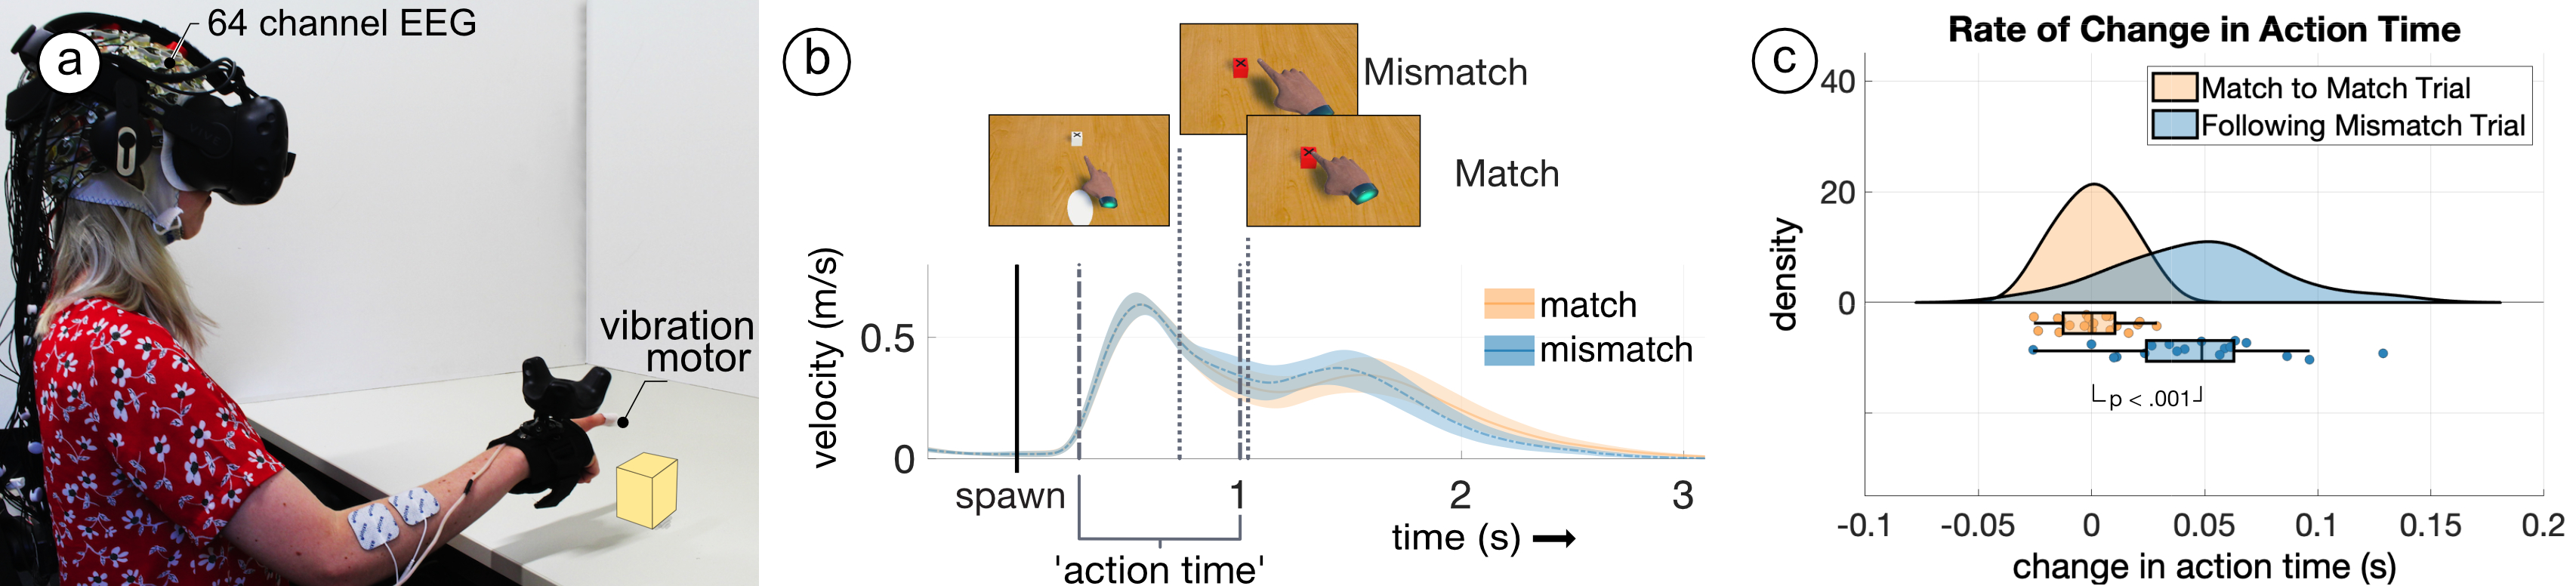
\includegraphics[width=\textwidth]{figures/task_behavior.jpg}
  \caption{Task Structure and hand velocity profile. \textbf{A} Participants were instructed to reach to an appearing cube on a desk in front of them. They were equipped with a VR, a 64 channel EEG cap, electrode spacers and rigid body tracker on the hand. The vibration motor was placed under the fingertip of the index finger. \textbf{B} Top: Inside VR view of experimental scene. Bottom: Grand-average velocity with 95\% confidence interval of both, match and mismatch conditions with event markers for object `spawn', `action time' start and end as well as moments of object touch in match and mismatch conditions. \textbf{C} Distribution of \textit{rate of change} in `action time' between two subsequent match trials and following a VR glitch. A dot represents the average per participant per condition.}
  \label{setup_and_behavior}
\end{figure}

\subsection{Prolonged `Action time' Following VR Glitches}

`Action time', the hand movement period from movement start to reaching the object, lasted on average .74s (SD = .15) in match- and .69s (SD = .15) in mismatch trials. 

% Adding vibrotactile stimulation did not affect hand movement profiles ($b=-.01, t=-1.7, p=.1$) and neither did the interaction of congruity and vibrotactile stimulation ($b=.02, t=1.8, p=.07$). Hence, as with the EEG analysis we pooled trials ignoring the feedback modulation.

We calculated the \textit{rate of change} in `action time' as a metric of post-error slowing. Following match trials, `action time' in the subsequent trial did not change, i.e. 0s (SD = .02). However, following mismatch trials, `action time' was increased in the subsequent trial on average by .05s (SD = .04); this modulation was about 48 times more likely to occur under the model considering mismatch modulation than the null model (equivalent ${\chi}^2_{(1)} = 48.1, p<.001$), see figure \ref{setup_and_behavior}c. 

% Adding vibrotactile feedback did not affect post-error slowing significantly ($b=-.02, t=-1.4, p=.15$). 

Using the trial-to-trial adaptation in `action time', trial classes (match/mismatch) were classified with an average within-subject classification accuracy across folds of 55.4\% (SD = 4.8), remaining below the significance threshold of the simulated chance level at 63.4\% (SD = 0.6).

\footnote{For completeness, we also report a classification scheme using behavioral data of all trials, maintaining unequal trial numbers per match and mismatch condition. We found that using data from all trials and maintaining unequal class sizes increased the classification to 67\% accuracy. See the supplementary material for more detail.}









%%%% writing resources
% Frage: wenn vel profiles mit movement onset aligned dann sollten evtl. kurven gleich sein, es sei denn es gibt einen "kontinuierlichen" rekalibrationseffekt ist in den syncs. mit drin
% im idealfall ist der rekalibrationseffekt 1/4 der 300ms
% Optimierungsprozess um den RMSE bei rekalibration zu optimieren
% mallot VR noise adaptation
% The addition of a haptic sensation while touching the virtual objects (by means of vibrotactile stimulation) led participants to generally move their hand slower during the whole trial, see \ref{setup_and_behavior} C middle row. Participants started their outward movement earlier and their outward peak magnitude was lower when approaching the target (for example at 50 ms preceding object selection, $t_{18} = -2.14, P = .03$). Following trials with spatio-temporal asynchrony, movement behavior was altered in the next trial. An earlier movement onset with a broader peak and immediate retraction following object select was observed (for example at 100 following object selection, $t_{18} = -17.24, P = 0$). Taken together, the task introduced spatio-temporal asynchrony, with rendered vibrotactile feedback as well as the asynchrony impacting future reaching movement characteristics.
\subsection{Localizing sources linearly discriminating synchronous and asynchronous events based on ERPs}
With an across-participants average classification accuracy of ~78 percent the linear discrimination between asynchronous and synchronous trials exceeded chance level at \~56 percent, $t_{18} = 42.1, P = 0$. In the fourth (200-250 ms) and sixth (300-350 ms) time window post event the control signal, that is channel activity weighted by classification weights, showed a clear separation between classes, see \ref{lda} B and C.
% the ttest against simulatedchance is kinda weird
% check ~ sign in latex
% is lda control signal well explained or is it over irrelevant for the paper
\begin{figure}[h]
  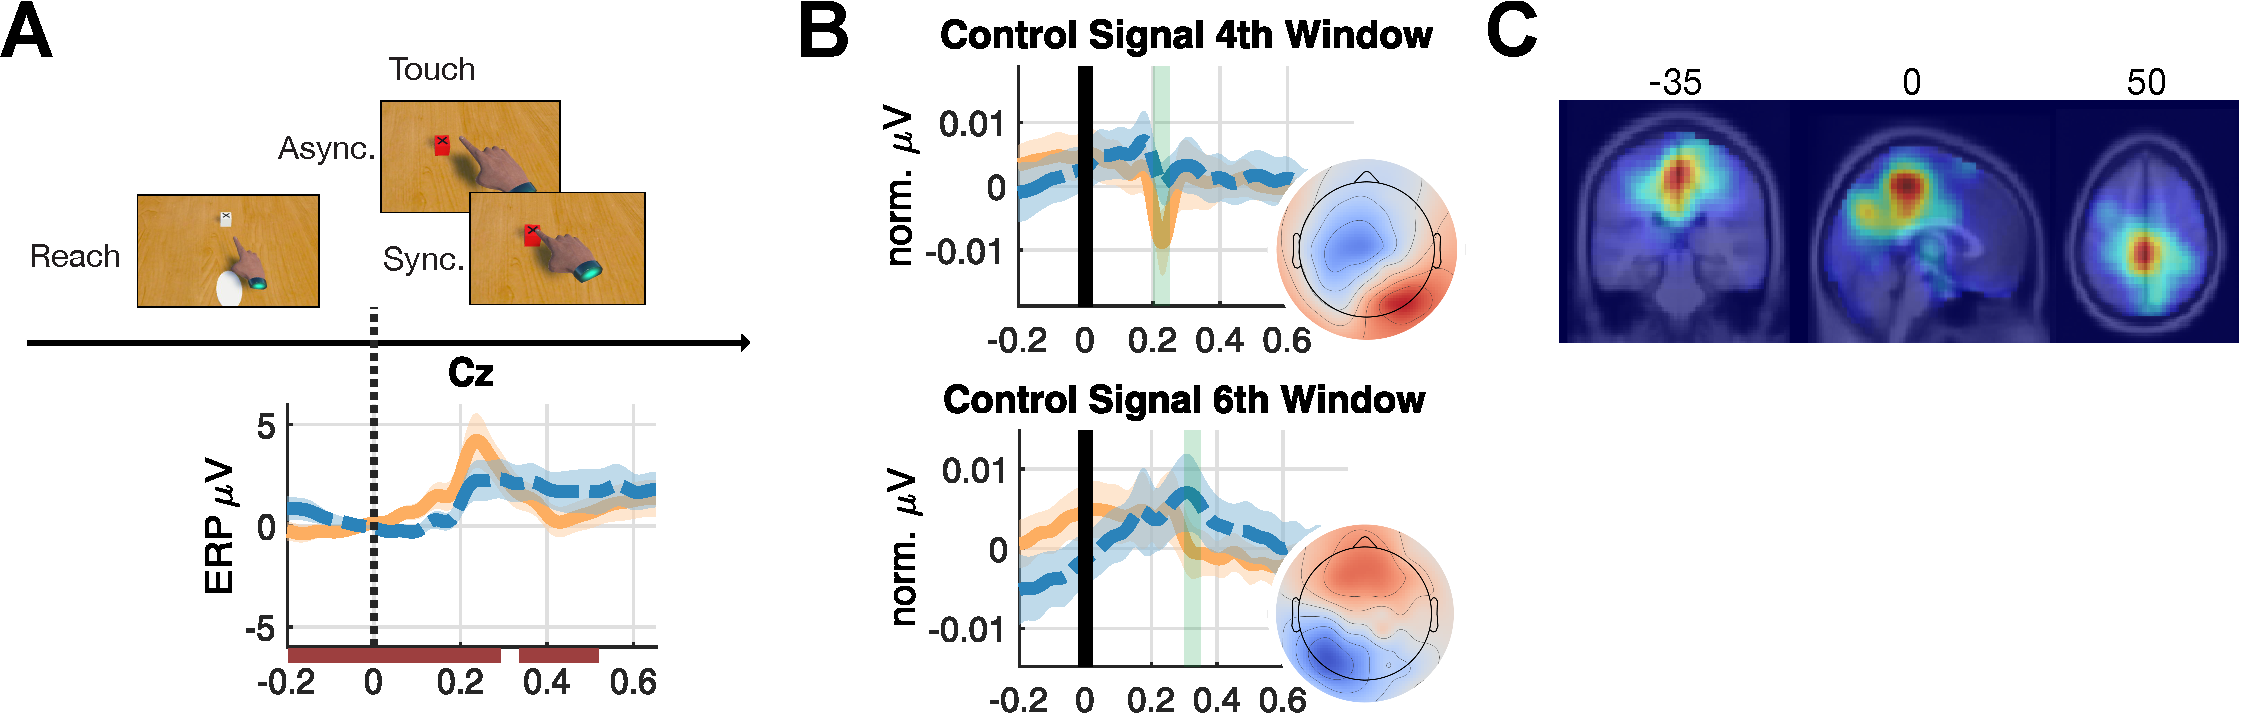
\includegraphics[width=\textwidth]{figures/fig2_discrimination_short.pdf}
  \caption{\textbf{A} An LDA classifier was trained on eight windowed means of 50 ms size from 50 to 450 ms following object selection. Two classes of synchronous and asynchronous trials were labeled for training and cross-validation. Bottom, grand-average ERP of projected source mixture at electrode Cz with significant class differences marked. \textbf{B} Grand-average ERP projected through sources of focus in the 4th and 6th time windows respectively with scalp map of control signal activity. \textbf{C} Localization of focused sources on average across all time windows used to determine seed for region of interest clustering of independent components.}
  \label{lda}
\end{figure}
With the goal to employ the trained BCI classifier for neuroscientific inquiry, we investigated which EEG effective sources contributed maximally to the classification. This source reconstruction serves two purposes: (1) Asserting that the classifier does not rely primarily on artifactual EEG sources, and (2) gain additional information about the contributing brain regions to allow neuroscientific interpretations. Across all time windows, a prominent source location contributing maximally to the classification was identified in the brain at a central-parietal location (MNI X = 0, Y = -35, Z = 50).

% were most relevant to the classification, a central-parietal (MNI X = 0,Y = -35,Z = 50) as well as an right lateralized occipito-parietal (MNI X = 20,Y = -65,Z = 30) location, see \ref{lda} E and F.
\subsection{Independent component clustering and grand-average ERSP}
We used the above result as a region of interest (ROI) seed for the repetitive cluster optimization approach. This resulted in a cluster solution containing an optimal central-parietal cluster with a centroid location around X = -2,Y = -37, Z = 46 (MNI), a mean residual variance of 5\%, containing 17 of 19 participants and 21 independent components. Providing an overview for the cluster of interest, the grand-average time-frequency characteristics are a useful guide for the following single-trial investigation. In the grand scheme, the task elicited increased theta-band activity following the appearance, or spawn, of the target to be selected ($t_{16} = 4.02, P = 0$ at -300 ms and 5 Hz). A similar theta-band signature, albeit to a lesser extent, was observed following spatio-temporal asynchronous object selection indicated by color change and vibration in the vibrotactile trials ($t_{16} = 2.16, P = 0.02$ at 270 ms and 4.5 Hz). Further, theta-band activity exceeded baseline activity during the randomized interval leading up to the object spawn. Significant alpha- and beta-band power decrease was observed during the trial hand movement phase ($t_{16} = -3.37, P = 0$ at 0 ms and 12 Hz; $t_{16} = -5.87, P = 0$ at 0 ms and 21 Hz) as well as leading up to the object spawn, predominantly in the beta-band ($t_{16} = -3.85, P = 0$ at -2200 ms and 21 Hz). Beta-band power increase outlasted alpha-band power increase after ~1s following asynchronous object selection ($t_{16} = -4.22, P = 0.003$ at 1100 ms and 21 Hz), \ref{grand_average_ersp} B.
\begin{figure}[t]
  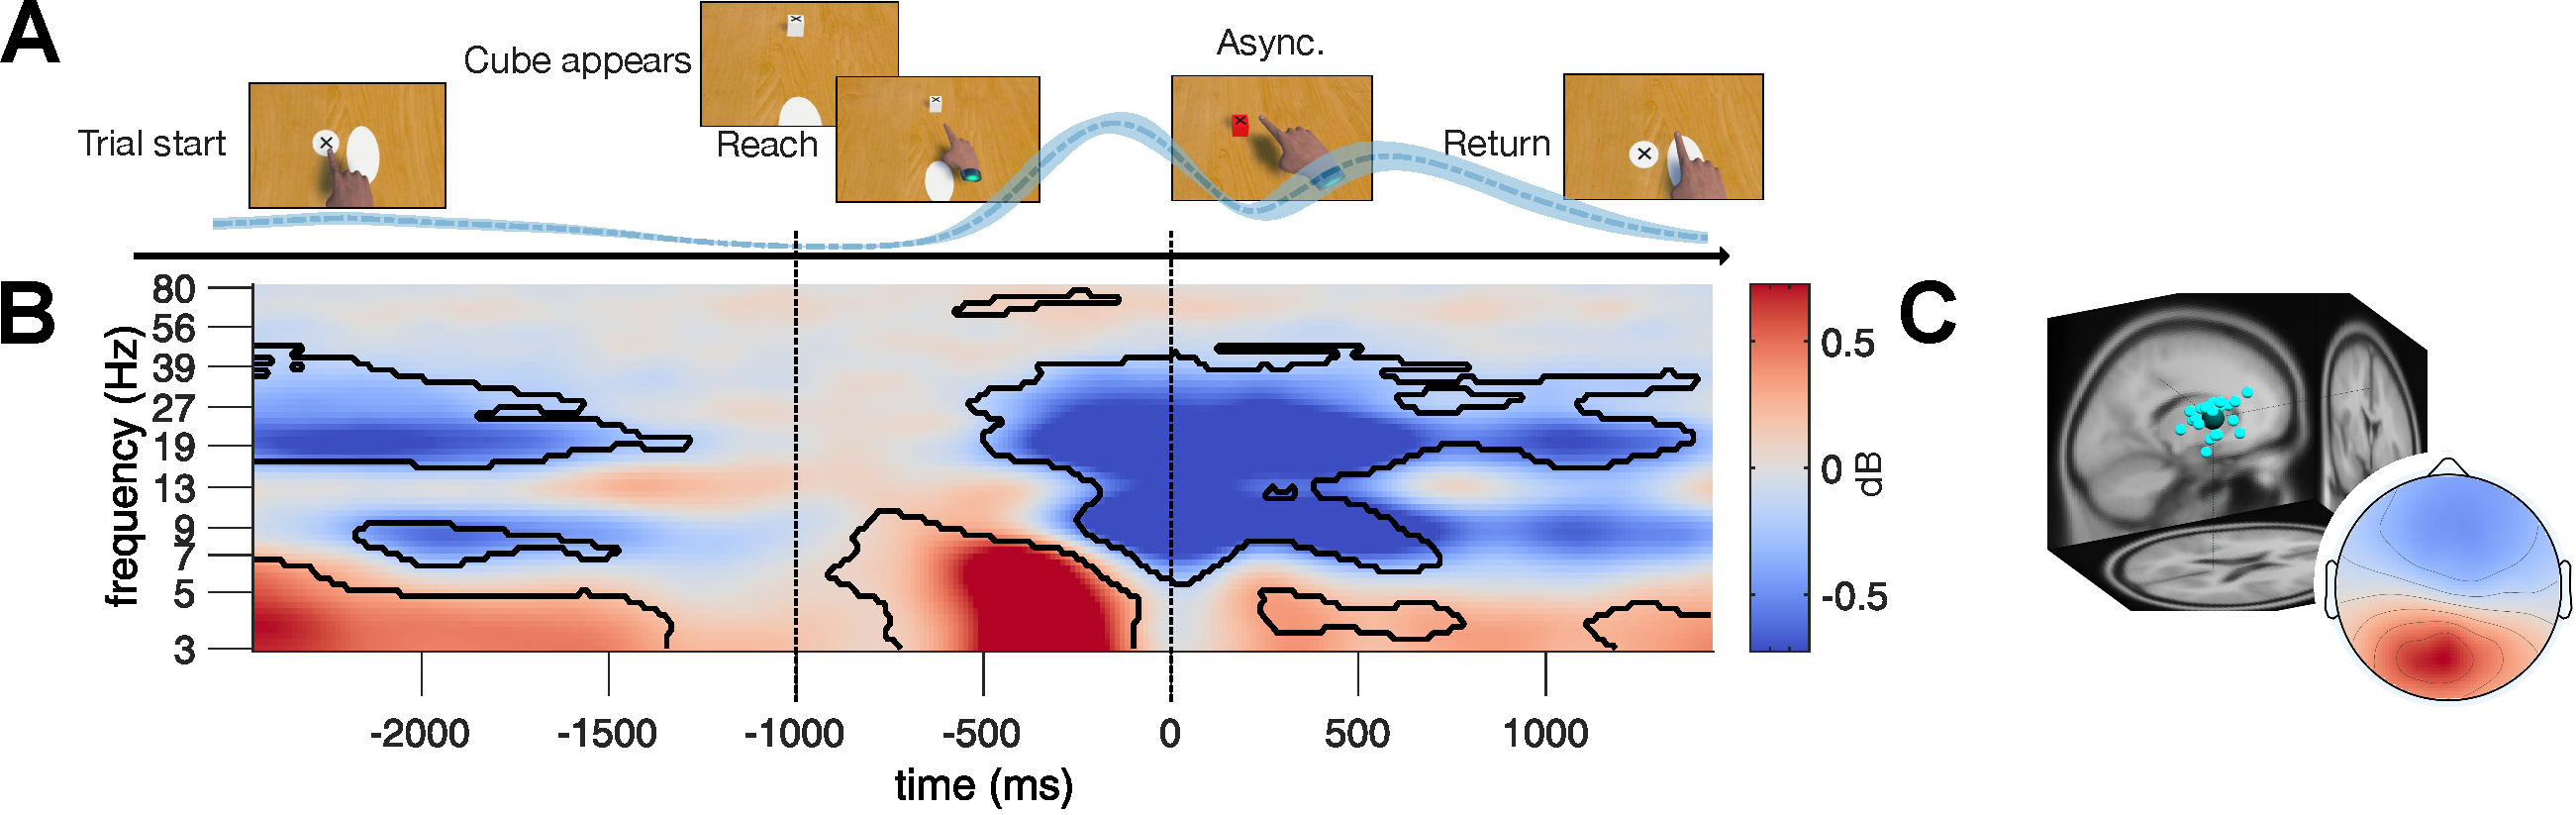
\includegraphics[width=\textwidth]{figures/fig3_context_grand-average_short.pdf}
  \caption{\textbf{A} Task and velocity profile of asynchronous trials. \textbf{B} Grand-average event-related spectral perturbations, that is changes in logarithmic scale over a divisive baseline. Black lines enclose areas of significant regions containing at least 50 pixels below P = .05 calculated using permutation t-tests. For visualization, time-frequency maps were smoothed with a Gaussian (width = 1.5). \textbf{C} Dipole of clustered independent components and the cluster mean scalp map of the optimal cluster seeded with LDA results.}
  \label{grand_average_ersp}
\end{figure}

%at X = 21,Y = -56, Z = 31 (MNI), mean residual variance of 7\%, containing 17 out of 19 participants and 18 independent components. Optimizing for the central-parietal ROI resulted in a cluster solution with an optimal cluster located around X = -2,Y = -37, Z = 46 (MNI) with a mean residual variance of 5\%, containing 17 of 19 participants and 21 independent components. There was no overlapping independent component present in both clusters. 
%In the right occipito-parietal cluster, a high alpha-band (12-18 Hz) power increase pre- and succeeded the hand movement phase, see \ref{grand_average_ersp} D and \ref{velocity} C top to bottom. 
\subsection{Providing context: single-trial regressions of haptic and velocity at moments of spatio-temporal asynchrony}
Figure \ref{st_ersp} B shows betas from single-trial regression including a baseline vector, whether physics were in part rendered through haptic feedback, hand velocity at the moment of spatio-temporal asynchrony, their interaction as well as the time elapsed since the object spawned. Low alpha-band during the baseline interval preceding object spawn positively impacted low-alpha band power preceding and following the object selection event ($t_{16} = 2.95, P = 0.003$ at 200 ms and 9 Hz post event), see \ref{st_ersp} B, C first column. Further, baseline beta-band power between 19-27 Hz impacted post event beta-band power in scattered clusters at 500 and 1000 ms post event. As expected, 50 Hz during baseline positively impacted 50 Hz band power during the trial hinting at the presence of line noise in some if not all independent components comprising the cluster.
% make sure the names are congruent throughout paper
% idea: separate RT measure in RT and 'action time' -> the time from spawn to movement start
% velocity -> slack in the system
% RT -> generelle "kognitive Aufmerksamkeit"
\begin{figure}[t]
  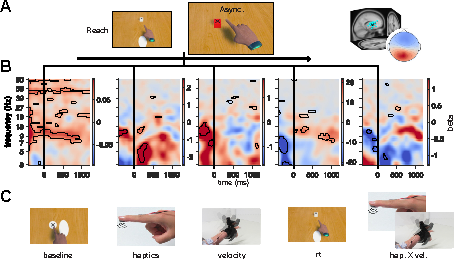
\includegraphics[width=\textwidth]{figures/fig4_ersp_single_trial_short.pdf}
  \caption{\textbf{A} Moment of spatio-temporal asynchrony. \textbf{B} Multiple regression coefficients, betas. Black lines enclose areas of significant regions containing at least 10 pixels below P = .05 calculated using permutation t-tests. For visualization, time-frequency maps were smoothed with a Gaussian (width = 1.5).} \textbf{C} Predictors.
  \label{st_ersp}  
\end{figure}
With increasing time elapsed between object spawn and object selection, reaction time, alpha-band power increased following visuo-spatial asynchronous object selection ($t_{16} = 1.96, P = 0.03$ at 250 ms and 12 Hz post event), see \ref{st_ersp} B, C fourth column. Preceding the event, reaction time negatively impacted a theta-band burst ($t_{16} = -2.91, P = 0$ at -200 ms and 7 Hz pre event). The two \textit{contextual} sensory predictors haptics and hand velocity at the moment of object selection as well as their interaction exhibited differential influence compared with baseline and reaction time predictors. Enabling vibrotactile stimulation increased theta-band power immediately following the moment of object selection ($t_{16} = 2.52, P = 0.02$ at 180 ms and 5 Hz post event). Further, enabling vibrotactile stimulation increased high alpha-band activity in a similar time window ($t_{16} = 2.58, P = 0.02$ at 180 ms and 12 Hz post event). Both enabling vibrotactile stimulation and increasing hand velocity increased alpha-band activity preceding object selection, exemplary for hand velocity ($t_{16} = 3.43, P = 0.003$ at -200 ms and 12 Hz pre event). Besides small, scattered clusters, hand velocity did not impact event-related spectral activity as a main effect. However, increasing hand velocity decreased theta-band power in a burst immediately succeeding object selection ($t_{16} = -2.05, P = 0.04$ at 180 ms and 4 Hz). Further, pre-event interaction effects indicated a decrease around the alpha-band with increasing hand velocity in vibrotactile trials only.

% discussion
%\section{Discussion}% start with summary
% aim for 1500 - 2000 words

% Points to discuss
% - is classification success dependent on level of haptic immersion? -> cite that it also works better in meditators for example

Coherent multisensory integration yields meaningful perceptual experiences and is central to adaptive behavior because it allows animals to perceive a world of coherent perceptual entities. In this work, we present evidence for neural signatures originating in central-parietal EEG sources during a spatio-temporal multisensory binding challenge. In order to carve out a signal separating cases of spatio-temporal synchrony from asynchronous cases we employed brain-computer interface technology. Through localization of the classifier weights we gained access to a node in the hierarchical inference network. Subsequent single-trial analysis on the spectral signatures exhibited a separation of alpha- and theta-band characteristics. In the time-domain, the signature can be employed for human-computer interaction purposes as we have shown it is accurately classifiable in two classes. Further, we functionally distinguished theta-band activity from alpha-band activity using single-trial regression. Alpha-band activity following spatio-temporal asynchrony was predicted by baseline activity as well as reaction time, the time elapsed to reach for the target. Both predictors allude to the general temporal task structure and hence may be separated from instantaneous processing. On the other hand, theta-band burst succeeding a binding challenge referred to the multisensory context, that is rendered physics and its interaction with the instantaneous hand velocity.


% maube good conclusion?
Adding to the significant body of evidence about (bayesian) prediction error computations, our findings enable targeted signal acquisition for neural interface technology in VR. 


%%%% writing ressources below
% - discuss reasons for low R^2 and approaches to address it (experiment design and methods (unfolding other processes, adding regressors etc.)) is there a meta study on effect sizes in timefrequency resolved EEG studies. What does Johanna report, regarding effect size?
% - is proprioceptive feedback important in our task: I'd argue against that because I consider vibration on the fingertip to be an exteroceptive sensation and do not consider it relevant where the hand was and how my joints were angled etc. during the mismatch event, therefore i stick to exteroceptive prediction errors only!
% - On world stability: designing visuo-haptic mismatches in virtual environments means further complicating the action-perception cycle understood as hypothesis testing. By pseudo-randomizing when one of the 25 percent chance oddballs appears, hypothesis testing and subsequent evaluation of the latent variables causing the oddball to appear becomes meaningless.

% then summarize results as below paper claim:
%(touch epochs)
%1. LDA location: Central-parietal EEG source activity discriminates between predicted and perturbed visuo-haptic perceptual experiences, in our case the touching of a cube on a desk, baring similarities to a classical simon task.
%(full epochs)
%2.1. ICs clustered to the centroid of the weighted ICs contributing the strongest to the LDA classifier were located to an area between precuneus and posterior cingulate cortex.
%2.2. Hand velocity characteristics, an event-related potential as well as an event-related spectral signature were explained by adding a haptic channel, increasing the level of immersion in the perceptual experience.
%2.3. Further, we observed responses locked to the feedback onset independent of differences in ongoing motor behavior between matching and mismatching classes. (description-level)
%(touch epochs)
%3.1. IC source dynamics following a visuo-haptic perturbation differ from predicted perceptual experiences (see 1., show difference erp and ersp)
%3.2. Following a visuo-haptic perturbation, the context of said perturbation operationalized by hand velocity, haptic feedback and their interaction, impact IC source dynamics only faintly.
%(next trial epochs)
%4. Post perturbation behavioral adaptation is in line with previous findings and may be explainable through reinforcement learning like computations in the brain.

% 1. start with a summary of the most important results
% -> what was the goal of this research?
% 2. situate findings in literature
% -> challenges for mobi research and how to make stimuli more salient
% -> bodily self perception
% 3. link back to introduction and papers cited in introduction

%so there are 2 things participants do in the task: 
%1. they collide too early and immediately adapt hand movement and have mmn / frontal theta -> Prediction Error
%2. they do RL using PE signal and adapt subsequent behavior (trial after mismatch)

% some arguments why ERP:
% - see Cohen 2014 muscle twitches: In our final set of analyses,we examined the ERPs—the time-domain EMG onset-locked EEG potential. Thiswas done mainly to replicate previous findings concerning the relationship between the ERP and partial errors.
% - moving towards an applicable metric to detect things online, hence must be computationally inexpensive, therefore ERPs
% - use ERP section as exemplary for understanding results
% - In haptically richer environments, processing gets more accurate and hence amplifies the error signal originating in or near anterior cingulate cortex (ACC). Moving fast and experiencing richer haptic feedback impact error processing
% - how does erp and ersp correlate. gamma and n200 occipital etc. filtering low frequency for erp does not mean higher ERSP frequency burst might not add to slow cortical ERPs -> therefore, approach is valid

% - discuss with spatial conflict processing: Savoie, & Simon Task results: cohen, cavanagh, toellner
% - reference to self and body ownership, spatial computations between egocentric and allocentric? cite Ehrsson, Slater, Gonzales-Franco (uncanny valley of haptics)
% - single-trial regression challenges in mobile brain body imaging studies: energy of stimulus, Time-locked vs. continuous regressors/stimuli, EEG artifacts due to movement, Contrast desktop stimulation vs. wide FOV in VR, Higher cortical noise, Saliency of stimulus, necessary attention on stimulus %in terms of predictive coding,
% - Study specific shortcomings: low N, both in subjects and in trials due to oddball paradigm
% - assume frontal evaluation of asynchronoy guiding future action and therefore did bot correlate any EEG metric with a post-error slowing parameter.
% - IC sources located near posterior cingulate cortex may anchor the self in the afforded reference frame, providing grounds for spatial predictions during ongoing perceptual experience.
%% discuss reasons for low R^2 and approaches to address it (experiment design and methods (unfolding other processes, adding regressors etc.)) 
% is there a meta study on effect sizes in timefrequency resolved EEG studies. What does Johanna report, regarding effect size?

\subsection{Challenges and opportunities investigating free moving navigators}
Energy of the stimulus 

\subsubsection{Time-locked vs. continuous regressors/stimuli}
\subsubsection{EEG artifacts due to movement}
\subsubsection{Contrast desktop stimulation vs. wide FOV in VR}
\subsubsection{Higher cortical noise}
\subsubsection{Saliency of stimulus, necessary attention on stimulus} %in terms of predictive coding
\subsubsection{Study specific shortcomings}
low N, both in subjects and in trials due to oddball paradigm


% methods
\section{Materials \& Methods}
The objective of our study was to explore EEG and movement signature with the potential to detect visuo-haptic conflicts in VR. As such, we designed a study in which participants perform a 3D object selection task in VR (modeled after~\cite{singh_visual_2018}). As a participant reaches out to touch an object, they were presented with three sensory feedback modalities (a visual baseline, tactile and tactile with force-feedback). However, to provoke the participants' brains into processing an unrealistic VR interaction, we sometimes provide the feedback prematurely. 

In this paper, we excluded trials with force-feedback. They were only collected for a subset of the participants and were always presented following the counterbalanced conditions of visual baseline and tactile. Therefore, the force-feedback condition did not impact the the visual and tactile contrast and the results including force-feedback are reported elsewhere~\cite{Gehrke2018}. However, for completeness, we chose to include the descriptions of the force-feedback setup in the following descriptions.

\subsection{Apparatus}
The experimental setup, depicted in Figure~\ref{setup}, comprised: (1) a VR headset and a wrist-mounted wearable VIVE tracker, (2) a 64-channel EEG system, (3) one vibrotactile actuator worn on the fingertip, and (4) a medically-compliant EMS device connected via two electrodes worn on the forearm for a subset of participants.

\begin{figure}[!ht]
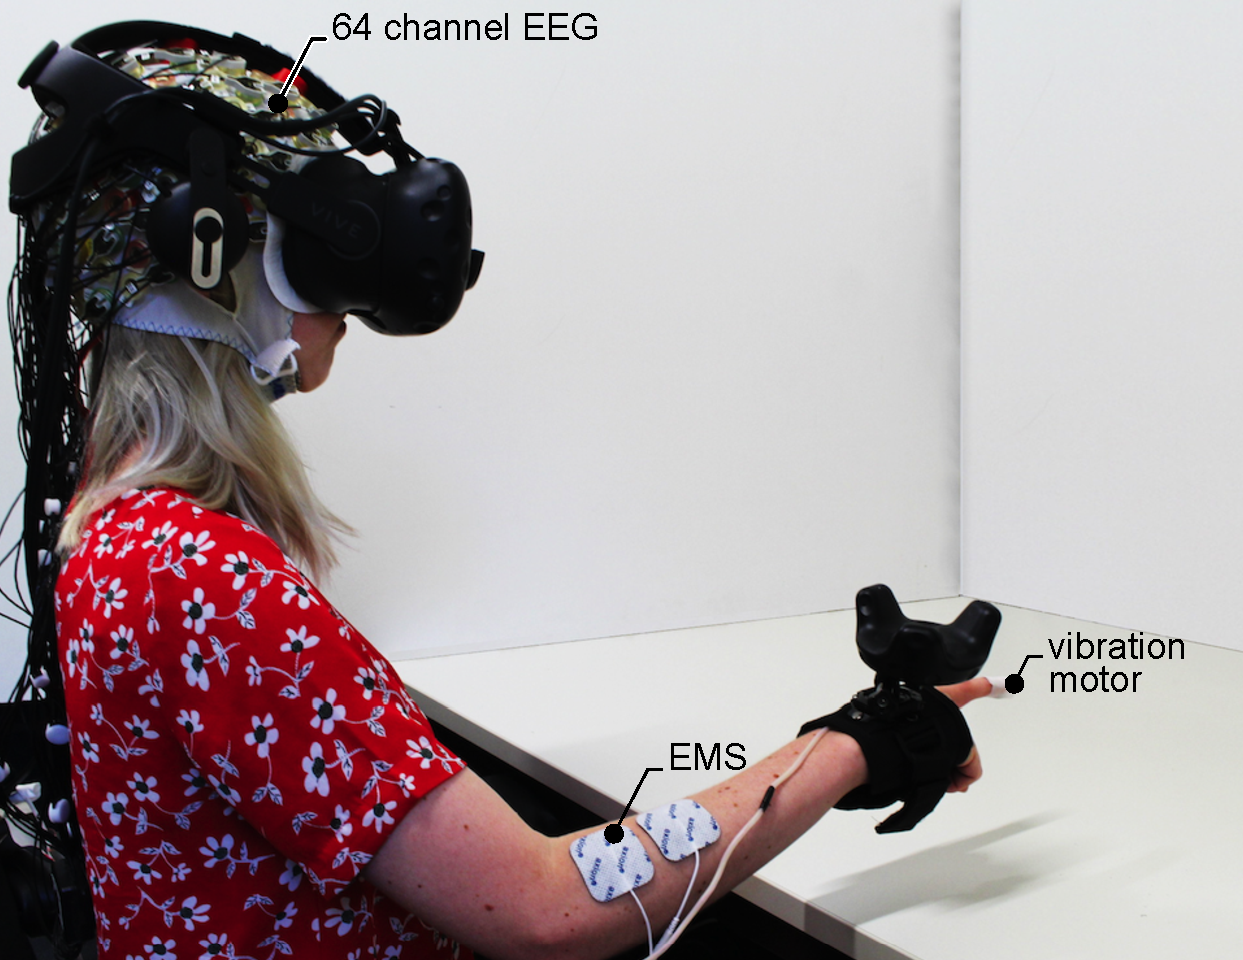
\includegraphics[width=\linewidth]{figures/experiment.pdf}
%\missingfigure[figcolor=white]{Shows setup.}
%\vspace{-17pt}
\caption{Our experimental setup (image with consent from participant).}
\label{setup}
\end{figure}

\textbf{(1) VR and hand tracking.} We used an HTC Vive headset (HTC Corporation, Taoyuan, Taiwan) with the Vive Deluxe Audio Strap and custem EEG cap spacers \footnote{https://grabcad.com/library/adapter-for-vr-eeg-setups-1} to ensure a good fit and less discomfort due to the EEG cap. We used a Vive Tracker, attached to the participant's wrist, to track their right hand. 

\textbf{(2) Vibrotactile feedback.} We used a vibration motor (Model \textit{308-100} from \textit{Precision Microdrives}), which generates 0.8g at 200Hz. This motor measures 8mm in diameter, making it ideal for the fingertip. The vibration feedback was driven at 70mA by a 2N7000 MOSFET, which was connected to an Arduino output pin at 3V.

\textbf{(3) Force feedback.} We actuated the index finger via electrical muscle stimulation (EMS), which was delivered via two electrodes attached to the participants' \textit{extensor digitorum} muscle. The finger actuation was achieved via a medically-compliant battery powered muscle stimulator (\textit{Rehastim} from \textit{Hasomed}), which provides a maximum of 100mA and is controllable via USB. 

% We utilized the extensor digitorum since we found that we can robustly actuate it without inducing parasitical motion of neighboring muscles; this was verified during pilot studies. This finger actuation was achieved via a medically-compliant battery powered muscle stimulator (\textit{Rehastim} from \textit{Hasomed}), which provides a maximum of 100mA and is controllable via USB. We chose this device since it had been successfully used by researchers as a means to generate force feedback in both VR~\cite{lopes_walls_2017} and AR~\cite{lopes_AR}. The EMS was pre-calibrated per participant to ensure a pain-free stimulation and robust actuation. 

\textbf{(4) EEG Setup.} EEG data was recorded from 64 actively amplified electrodes using BrainAmp DC amplifiers from BrainProducts. Electrodes were placed according to the extended 10\% system ~\cite{oostenveld_five_2001}. After fitting the cap, all electrodes were filled with conductive gel to ensure proper conductivity and electrode impedance was brought below 5kOhm for all electrodes. EEG data was recorded with a sampling rate of 1000 Hz. We synchronized tracking, EEG data, and an experiment marker stream that marked sections of the study procedure using labstreaminglayer\footnote{https://github.com/sccn/labstreaminglayer}.

\begin{figure*}[!ht]
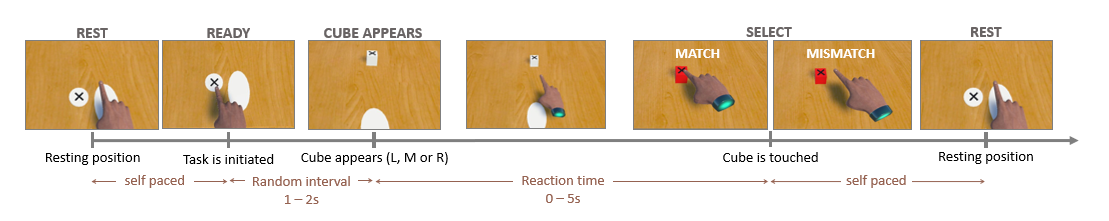
\includegraphics[width=\linewidth]{figures/Task_mismatch.PNG}
\vspace{-15pt}
\caption{Interaction flow depicting one trial in our 3D object selection task.}
\label{task_flow}
\end{figure*}

\subsection{Training phase}
We asked participants to wear the HTC VIVE VR headset for a maximum of 24 trials practice trials. Overall, the EEG fitting, calibration, and practice trials took around 30 minutes (with two experimenters).

\subsection{Task}
Participants performed a 3D object selection task in VR design with Unity Software (Unity Technologies, San Francisco, USA). The interaction flow of our task, depicted in Figure~\ref{task_flow}, was as follows: (1) participants moved their hands from the \textit{resting position} to the \textit{ready position}, to indicate they were ready to start the next trial; (2) participants waited for a new target to appear (the time of a new target spawning was randomized between 1-2 s); (3) then, the target (a cube) would appear in one of three possible positions (center, left, right), all equidistant from the participant's \textit{ready position}; (4) then, participants acquired the target by moving and touching the target with their index finger. (5) After a target was acquired, participants moved back to the \textit{resting position}. Here, they could take a break before the next trial.

\subsection{Interface conditions}
Participants performed the task in three additive feedback conditions:

(1) \textbf{visual-only (Visual)}: when participants touched the cube, it changed its color from white to red (visual feedback)
% ; our no-haptics \textbf{baseline}~\\
\indent(2) \textbf{tactile (Vibro)}: when participants touched the cube in the vibro condition, they received a 100 ms vibroactile stimulus and the color change (visual + tactile feedback)
% ; this is the only available haptic feedback in today's VR experiences.~\\
\indent(3) \textbf{force-feedback (EMS)}: in this condition, participants also received a 100 ms of EMS stimulation at the index finger extensor in addition to the visual and vibrotactile feedback (visual + tactile + force feedback)
% . As prior research showed the EMS stimulation of the opposing muscle (in our case, the extensor) is perceived as the resisting force that arises from pushing against the cube (i.e., force feedback)~\cite{lopes_muscle-propelled_2013,lopes_walls_2017,lopes_impacto:_2015}.

% We designed our three feedback conditions additively because additional haptic feedback is generally associated with more haptic realism, therefore, we hypothesized that ERPs would demonstrate some correlation to the ascending level of the feedback's realism.

\subsection{Introducing Visuo-Haptic Mismatches}
To allow us to compare the event-related EEG and movement signatures in a realistic vs. unrealistic interaction, we presented participants with two different classes of trials: \textbf{match trials (C)} (75\% of the trials) and \textbf{mismatch trials (M)} (25\%). This procedure elicits a prediction mismatch signal in 25\% of the trials similar to previous designs investigating the impact of target probabilities~\cite{polich_updating_2007}.  %on ERP modulations
In the \textbf{matching} trials, the feedback stimuli were presented upon touching the object, exactly when participants expected them to occur based on the available visual information (finger touching the target). In contrast, in the \textbf{mismatch} trials, the feedback stimuli were triggered prematurely, which was accomplished by enlarging the invisible radius of touch detection by 350\%. While in the match trials, we used a cube collider of the exact size of the VR cube, in the mismatch trials, we used a larger sphere collider. Our collider enlargement was based on the study design by Singh et al.~\cite{singh_visual_20008}, in which they showed that VR users can detect a visual mismatch at around 200\% of offset from the target. In our pilot tests, we decided to extend the offset to 350\% to make the mismatch more obvious so as to provoke more pronounced prediction errors. 

Also, we used a match-to-mismatch ratio of 75\%-25\% of the total trials by modeling our study after previous studies, which also ensure that participants are faced with a detectable unrealistic behavior of the virtual environment~\cite{Liao2011,Wiersema2007,Donchin1988}. For these unrealistic trials to occur, the participants must first be able create a stable model of how the VR world operates, thus the VR world cannot behave at a random 50\%-50\% match-mismatch ratio.

Finally, these match vs. mismatch trials were presented in five randomly generated sequences, each with an equal distribution of matches and mismatches.

\subsection{Experimental design}
The experiment consisted of five phases: (1) a setup phase; (2) a calibration phase; (3) a short training phase; (4) the task itself, in all three possible interface conditions, each followed by a subset of items from the IPQ questionnaire (G1, REAL2, SP4 and INV1)~\cite{T.W.Schubert2003} and the NASA-TLX~\cite{Hart1988}. Lastly (5) participants were asked about their experience in the VR and which condition they enjoyed the most.

% For completeness, at the end of each condition we presented the four most relevant questions from the standard IPQ~\cite{ipq_paper}, in particular: G1, REAL2, SP4 and INV1. However, our hypothesis was that the inclusion mismatch trials, which were presented in 25\% of the cases, would lower the IPQ ratings dramatically.

We used a within-subjects design with 300 trials for each, the Visual and Vibro feedback condition, and 100 trials for the EMS condition. The order of the Visual and Vibro conditions was randomized across participants with the EMS condition always being the last block. 
% This was done to avoid potential overshadowing of the EMS stimulation (a very strong sensation) on the two other stimulation conditions.





%%%%% resources:
% \subsection{Task and Procedure}
% Using an HTC Vive VR Headset with the Vive Deluxe Audio Strap and a Vive Tracker (HTC Corporation, Taoyuan, Taiwan) attached to the right hand, a 3D object selection task was presented on a virtual table placed on an infinite white plane. The virtual environment was created in the Unity3D engine (Version, company details). White cubes appeared at random either in the center, to the left, or to the right of the participant, equidistant from a starting position (see Figure ??). The time of a new cube spawning was randomized between 1-2 seconds after starting a trial. 

% %no subsections? This so hard to parse, make a task heading or so?
% Participants were tasked to select the cube with their index finger and, upon completion, move their hand back to a resting position indicated on the table. The task was completed in two blocks of 300 trials each, with one block providing visual-only feedback, i.e. the cube changing its color from white to red upon selecting, and one block providing visual-tactile feedback, in which the selection contact was indicated by the color change plus a small vibrotactile pulse. Placed under the index fingertip, a vibration motor (Model \textit{308-100} from \textit{Precision Microdrives}), generating 0.8g at 200Hz and measuring 8mm in diameter was driven at 70mA by a 2N7000 MOSFET connected to an Arduino output pin at 3V. An initial 24 trial training session was followed by the two experimental blocks (balanced across participants), each followed by two questionnaires, NASA-TLX and IPQ. For the main experimental manipulation of asynchrony, 25\% of the trials (totalling 75 asynchronous trials per feedback block of 300 trials) exhibited spatio-temporal asynchrony in line with established oddball paradigms. Object selection was triggered prematurely by bounding a spherical collider to the cube and enlarging it by 350\% in comparison to a collider bounded to the shape of the cube in the synchronous trials. Asynchronous trials were sorted in a pseudo-randomized sequence following synchronous trials, i.e. between one and five synchronous trials preceeded an asynchronous trial. Extended task and apparatus descriptions can be found elsewhere \cite{Gehrke2019}.
% % todo add movie, figure and references
\subsection{EEG Preprocessing and Independent Component Analysis (ICA) \textcolor{green}{Lukas, Marius, Klaus}}
EEG data preprocessing and ICA were performed with Matlab 2019b (MATLAB, The MathWorks Inc., Natick, MA, USA), using the EEGLAB toolbox \cite{Delorme2004a} and our 'BeMoBIL Pipeline' scripts and functions. The single subject data was lowpass filtered with 124Hz and down-sampled to 250Hz. Channels which were contaminated with artifacts were automatically rejected using the PREP pipeline \cite{Bigdely-Shamlo2015} 'FindNoisyChannel' function, which is selecting bad channels by amplitude, the signal to noise ratio and correlation with other channels. Rejected channels were then interpolated while ignoring the EOG channel, and finally re-referenced to average reference (data A). The data was then filtered with a 1 Hz highpassfilter (data B), a first adaptive mixture independent component analysis, AMICA \cite{Palmer2011}, was used to identify eye related independent components (ICs) which were projected out of the sensor data (data A). For this, the rank was reduced by one for average reference use and further by the number of interpolated channels in the respective data set. To identify eye components IClabel  \cite{Pion-Tonachini2019} was used, whereas components exceeding a value of 0.7 for the 'eye' class were defined as eye components. Then, to detect segments of noisy data, an automated time domain cleaning (see \citet{Gramann2018}) on the time domain was performed on narrowly filtered data from 1 to 40 Hz. The data was therefore first split into 1 second long segments for which the mean absolute amplitude and standard deviation of all channels as well as the Mahalanobis distance of all channel mean amplitudes were calculated. All three methods results were then joined together in order to rank all segments. The 12\% highest ranking noisy segments were selected for rejection and an additional buffer of $+/-$ 0.49 sec was added around each segment resulting in about 15\% rejected data for each subject. This data was rejected from data B and a second AMICA was calculated on this time domain cleaned data. A dipole fitting procedure was performed for each spatial filter using the 10-20 standard electrode locations and a boundary element head model (BEM) based on the MNI brain (Montreal Neurological Institute, MNI, Montreal, QC, Canada). The spatial filter information was then copied back to the preprocessed, interpolated and average referenced data set (data A). Ultimatelty, all ICs with a 'brain' probability smaller than .5 as indicated by ICLabel were projected out of the data resulting in the final dataset of likely brain sources and their projections to the channels.
% todo bemobil pipeline citation/footnote

\subsection{Event-related Feature Extraction}
Data was epoched -3 to +2 seconds around the 600 \textit{cube selection} events and trials were removed (a) if the reaction time between cube \textit{spawn} and \textit{selection} exceeded two seconds or (b) large voltage fluctuations in the channels were detected via EEGLABs \textit{autorej} function. On average X trials were removed. % todo how many trials were removed 
For each remaining single trial we built event-related potentials for channels and independent components (ERP), event-related velocities, i.e. the magnitude of velocities in x, y and z direction (ERV) as well as event-related time-frequency decompositions (ERSP). Time-frequency decomposition were computed via the \textit{newtimef} function in EEGLAB for 3 to 80 Hz in logarithmic scale, using a wavelet transformation with 3 cycles for the lowest frequency and a linear increase with frequency of 0.5 cycles. Single-trial baseline vectors contained average power per frequency bin in the -200 to 0 ms window preceding cube \textit{spawns}. Where applicable, grand average ERSPs are computed by first averaging both trial data and baselines across trials in power then dividing trial data by baseline and transforming the outcome to logarithmic scaling. ERPs are plotted after bandpass filtering with a low and high cutoff at 0.1 and 15 Hz respectively.

\subsection{Classifier, Classifier Scalp Projections and Localization of Components relevant to Classification}
Following \citet{Zander2016} a regularized linear discriminant analysis classifier was trained per participant with all asynchronous trials constituting class 1 and a random sample of an equal size of synchronous trials labeled class 2. Using Matlab 2014a (MATLAB, The MathWorks Inc., Natick, MA, USA) with the open-source toolbox BCILAB ver. 1.4 the classifier was trained on windowed means as features. Therefore, average amplitudes of all channels and eight sequential 50 ms time windows between 50 and 450 ms following \textit{cube selection} were extracted following resampling to 100 Hz and band-pass filtering from 0.1 to 15 Hz. For robust performance estimation, a 5 x 5 nested cross-validation was used to calculate the classifiers reliability. Classification accuracy was statistically evaluated using a two-sample ttest with the mean classifier accuracy per participant across folds and simulated chance level given trial numbers in each class \cite{Muller-Putz2007}.

In order to learn what regions of the brain the classifier specifically relied on, we first transformed the LDA filters at each time window to LDA patterns reflecting a mixture of scalp activations with regards to the discriminative source activity \cite{Haufe2014a, Zander2016, Krol2019}. Subsequently, the relevance for classification can be computed using LDA filter weights per time window and the ICA umixing matrix. The equivalent current dipole models of independent compontents were then weighted by their relevance and ultimately visualized via EEGLAB dipoleDensity plots. We established the highest relevance voxel via visual inspection and used it as a seed region of interest (ROI) for group-level IC clustering. % maybe add movie for supplement material

\subsection{Clustering Independent Components for Group-Level Analyses}
To allow for group-level analyses across independent components, we clustered components based on their equivalent dipole locations (weight=6), grand-average ERSPs (weight=3), mean log spectra (weight=1), and scalp topography (weight=1), using a region of interest (ROI) driven repetitive k-means clustering approach \cite{Gramann2018}. The weighted IC measures were summed and compressed using PCA, resulting in a 10-dimensional feature vector for clustering. ICs were clustered by applying the k-means algorithm with k equaling the median number of ICs retained across subjects. ICs with a distance of more than three standard deviations from any final centroid mean were considered outliers. To ensure replicability of the clustering, we employed the same clustering approach reported in \cite{Gramann2018}. After applying desirable weights (number of participants: 2, ICs/participants: -2, spread: -1, RV: -1, distance from ROI: -2, Mahalanobis distance from the median: -1) the final clustering solution contained the ICs from X participants, a ratio of X ICs per participant, a spread of X, a mean RV of X\%, and a distance of X units in the MNI space for the cluster of primary interest.
% todo add clustering results and k
%\subsection{Single-Trial Regression and Multiple Comparison Correction using Threshold-Free Cluster Enhancement \textcolor{green}{Lukas, Marius, Klaus}}
% - mass univariate regression at the single subject level (Kutas rERP, Groppe, Pernet, Cavanagh, Cohen). Averaging betas and pvals, then do tfce transform on the mean and infer on the tfce statistic? \todo{check if this method correct, how did cohen do it?}
% - paired ttest with bootstrap-tfce multiple comparison correction \citep{SMITH200983} to make inferences about the interaction
% - Grand Average Statistics

% Submissions are not required to reflect the precise reference formatting of the journal (use of italics, bold etc.), however it is important that all key elements of each reference are included.
\bibliography{references}

\end{document}
